%% ****** Start of file aiptemplate.tex ****** %
%%
%%   This file is part of the files in the distribution of AIP substyles for REVTeX4.
%%   Version 4.1 of 9 October 2009.
%%
%
% This is a template for producing documents for use with 
% the REVTEX 4.1 document class and the AIP substyles.
% 
% Copy this file to another name and then work on that file.
% That way, you always have this original template file to use.

%\documentclass[aip,graphicx]{revtex4-1}
%\documentclass[aip,reprint]{revtex4-1}

%\usepackage{graphicx}

%\draft % marks overfull lines with a black rule on the right
%\documentclass[pre,aps,floatfix,authordate1-4,twocolumn]{revtex4-1}
%\documentclass[pre,aps,floatfix,authordate1-4]{revtex4-1}

\documentclass[aps,prl,superscriptaddress,twocolumn]{revtex4}



%\documentclass[aps,prl,preprint,groupedaddress]{revtex4}

\usepackage{rotating} 
\usepackage{times}
\usepackage{graphicx}
\usepackage{setspace}
\usepackage{amsmath}
\usepackage{epstopdf}
\usepackage[obeyFinal]{easy-todo}
\usepackage{csquotes}
\usepackage{xr}
\externaldocument{manuscriptPGPEsuppl}


\begin{document}

% Use the \preprint command to place your local institutional report number 
% on the title page in preprint mode.
% Multiple \preprint commands are allowed.
%\preprint{}

\title{NMRlipids IV: Headgroup \& glycerol backbone structures, and cation binding in bilayers with PE and PG lipids} %Title of paper

% repeat the \author .. \affiliation  etc. as needed
% \email, \thanks, \homepage, \altaffiliation all apply to the current author.
% Explanatory text should go in the []'s, 
% actual e-mail address or url should go in the {}'s for \email and \homepage.
% Please use the appropriate macro for the type of information

% \affiliation command applies to all authors since the last \affiliation command. 
% The \affiliation command should follow the other information.

\author{O. H. Samuli Ollila}
\email[]{samuli.ollila@helsinki.fi}
%\homepage[]{Your web page}
\affiliation{Institute of Organic Chemistry and Biochemistry,
Academy of Sciences of the Czech Republic, 
Prague 6, Czech Republic}
\affiliation{Institute of Biotechnology, University of Helsinki}


% Collaboration name, if desired (requires use of superscriptaddress option in \documentclass). 
% \noaffiliation is required (may also be used with the \author command).
%\collaboration{}
%\noaffiliation

\date{\today}

\begin{abstract}
% insert abstract here
  Primarily measured but also simulated NMR order parameters will be collected also for other than phophatidylcholine
  (these are discussed in NMRlipids I) headgroup. The information will be used to understand structural differences between 
  different lipid molecules in bilayers.
\end{abstract}

%\pacs{}% insert suggested PACS numbers in braces on next line

\maketitle %\maketitle must follow title, authors, abstract and \pacs

% Body of paper goes here. Use proper sectioning commands. 
% References should be done using the \cite, \ref, and \label commands


%\label{}
\section{Introduction}

PE and PG lipids are most common lipids in bacteria \cite{sohlenkamp16}.
Zwitterionic PE is the second most abundant glycerophospholipid in eukaryotic cells
and has been related to the diseases \cite{vance15,calzada16,patel17}.
Anionic PG lipids are less abundant, but is also proposed to be fundamental for terrestrial life \cite{furse17}.
PE and PG affect membrane protein functionality \cite{hariharan18} and bind to various proteins \cite{yeagle14}.
PE headgroup is also prone for negative membrane curvature and causes membrane fusion \cite{??}.
Therefore, the PE and PG headgroup structures play probably essential roles in 
many biological processes.

Structural details of lipid headgroups are mainly studied using NMR experiments, which
suggest that the glycerol backbone structures are largely similar irrespectively of the headroup \cite{gally81}, 
glycerol backbone and headgroup structure and behaviour are similar in model membranes and in bacteria \cite{gally81,scherer87,seelig90},
and the headgroup structures are similar in PC, PE and PG lipids, while headgroup is more rigid in PS lipids \cite{wohlgemuth80,buldt81}. 
%Extensive discussion about structural details of PE, PG or PS headgroups do not exists (as far as I know), 
%In contrast to PC lipids (see \cite{botan15} and references therein).
Some attempts to resolve conformational ensembles from NMR for PC lipids have been made,
but lesser extend for other lipids \cite{??}.
Classical molecular dynamics simulations could potentially give such ensembles and therefore enable
the detailed studies of lipid headgroup behaviour in complex biomolecular systems, but current
force fields are not accurate enough to reproduce the correct conformational ensembles for PC and PS headgroups \cite{botan15,antila19}.
Several MD simulations of PE and PG lipids have been published especially in the context of modeling
inner membrane of Gram-negative bacteria \cite{??}, but glycerol backbone and headgroup structures have not
been evaluated against experiments.

Besides the structure, also ion binding may regulate biophysical activity of especially negatively
charged lipid headgroups \cite{??}. Monovalent cation (except Lithium) binding to zwitterionic PC headgroups is
very weak, while multivalent ion binding is stronger but still weak \cite{??}. The ion binding affinity
data for PE is more scarce \cite{??}, but large differences to PC would be surprising.
Negatively charged lipids are suggested to bear same cation binding constants than zwitterionic lipids, but
the amount of bound ions to negatively charged membranes would still be larger because
the concentration of cations in the vicinity of membranes would be higher  \cite{seelig90}.
%is stronger
%Based on the electrometer concept and other data is has been suggested that \cite{seelig90}
%\begin{displayquote}
%  {\it ''(i) Ca$^{2+}$ binds to neutral lipids (phosphatidylcholine, phosphatidylethanolamine) and negatively charged lipids
%    (phosphatidylglycerol) with approximately the same binding constant of K = 10-20 M$^{-1}$; \\
%    (ii) the free Ca$^{2+}$
%    concentration at the membrane interface is distinctly enhanced if the membrane carries a negative surface
%    charge, either due to protein or to lipid; \\
%    (iii) increased inter-facial Ca$^{2+}$ also means increased amounts
%    of bound Ca$^{2+}$ at neutral and charged lipids; \\
%    (iv) the actual binding step can be described by a Langmuir
%    adsorption isotherm with a 1 lipid:1 Ca$^{2+}$ stoichiometry, provided the interfacial concentration C$_M$, is
%    used to describe the chemical binding equilibrium.''}
%\end{displayquote}
On the other hand, anionic PS lipids are proposed chelate with calcium ions \cite{??}.
In simulations, the cation binding affinity to PC and PS membranes is typically overestimated \cite{catte16,antila19},
which can be improved by applying the ECC to the partial charges of the force fields \cite{melcr18,melcr19}.

Here, we use open collaboration and order parameters of glycerol backbone and headgroup
to evaluate the accuracy of PE and PG heagroup structures, and the cation binding affinity
to anionic membranes containing PG lipids in the current MD simulation force fields.
The force field giving the best description for glycerol backbone and headgroup structures
of PC, PS, PG and PE headgroups (CHARMM36) reproduces the essential differences in order parameters
between these headgroups, and therefore enables the analysis of structural differences between the
headgroups.

%\begin{figure}[]
%  \centering
%  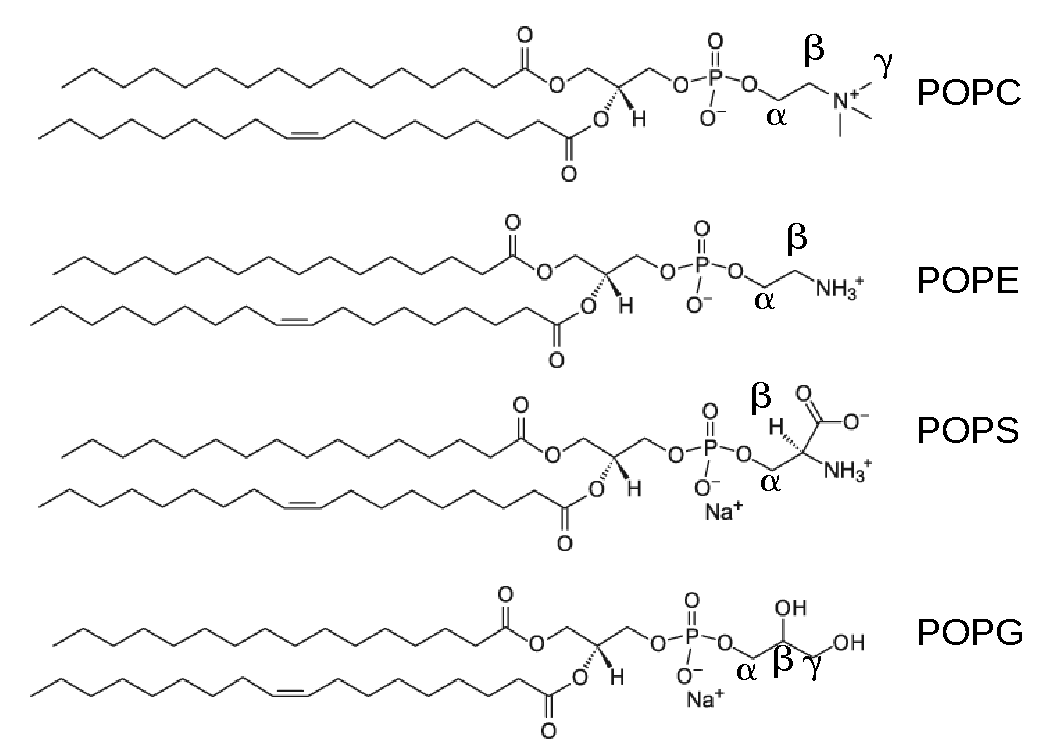
\includegraphics[width=9.0cm]{../Figs/lipids.pdf}
%  \caption{\label{lipids}
%    Chemical structures and labels for the headgroup carbons.
%  }
%\end{figure}



\section{Methods}
\subsection{Experimental C--H bond order parameters}% from the natural abundance $^{13}$C\,NMR}

The headgroup and glycerol backbone C--H bond order parameter magnitudes and signs of POPE and POPG
were determined by measuring the chemical-shift resolved dipolar splittings
with a R-type Proton Detected Local Field (R-PDLF) experiment~\cite{dvinskikh04} and
%The corresponding order parameter signs were measured with a
S-DROSS experiments~\cite{gross97} using natural abundance $^{13}$C solid state NMR spectroscopy
as described previously \cite{ferreira13,ferreira16,antila19}.
%The experiments were done in a Bruker Avance III 400 spectrometer operating at a $^1$H Larmor frequency of 400.03 MHz.
%Magic angle spinning (MAS) of the sample was used at a frequency of 5.15 kHz (R-PDLF experiment) and 5 kHz (S-DROSS experiment).
%The following experimental setups were used.
\todo{The rest of the details to be written. I am not sure how much we need to repeat the NMRlipidsIVps paper.}

\subsection{Molecular dynamics simulations}

Molecular dynamics simulation data were collected using
the Open Collaboration method \cite{botan15}, with
the NMR\-lipids Project blog (\url{nmrlipids.blogspot.fi}) and
GitHub repository (\url{github.com/NMRlipids/NMRlipidsIVotherHGs})
as the communication platforms.
The simulated systems are listed in 
Tables \ref{systems} (pure PE and PG bilayers without additional ions).
and \ref{systemsII} (mixtures and systems with additional ions).
Further simulation details are given in the SI, and
the simulation data are indexed in a
searchable database available at \url{www.nmrlipids.fi},
and in the NMRlipids/MATCH repository (\url{github.com/NMRlipids/MATCH}).

The C--H bond order parameters were calculated directly
from the carbon and hydrogen positions using the definition
\begin{equation}
S_{\rm CH}=\frac{1}{2}\langle 3\cos^2\theta -1 \rangle,
\end{equation}
where $\theta$ is the angle between the C--H bond and the membrane normal
(taken to align with $z$, with bilayer periodicity in the $xy$-plane).
Angular brackets denote average over all sampled configurations.
The order parameters were first calculated averaging over time separately
for each lipid in the system. The average and
the standard error of the mean were then calculated over different lipids.
Python programs that use the MDAnalysis library \cite{agrawal11,gowers16}
used for all atom simulations is available in Ref. \citenum{MATCHgit}
({\tt scripts/calcOrderParameters.py}). For united atom simulations, the trajectories
with hydrogens having ideal geometry were constructed first using either buildH program~\cite{buildH}
or ({\tt scratch/opAAUA\_prod.py}) in  Ref. \citenum{MATCHgit}, and the order parameters were
then calculated from these trajectories. This approach has been tested against trajectories
with explicit hydrogens and the deviations in order parameters are small \cite{buildH,piggot17}.
The ion number density profiles were calculated using the {\tt gmx density} tool
of the Gromacs sofware package \cite{gromacsMANUAL}.

\begin{table*}[htb]
  %\begin{sidewaystable*}[!p]
  \centering
  \caption{List of MD simulations with PE lipids.
    % The salt concentrations calculated as [salt]=N$_{\rm c} \times$[water]\,/\,N$_{\rm w}$, where [water]\,=\,55.5~M.
    % these correspond the concentrations reported in the experiments by Akutsu et al.~\cite{akutsu81}.
    % The lipid force fields named as in our previous work~\cite{botan15}.
  }\label{systems}
  \begin{minipage}[t]{\textwidth}
    \begin{tabular}{l c c r r r r r r c c}
      %\hline
      % some footnotes are not visible in typeset-MS (pdf)
      lipid/counter-ions & force field for lipids / ions  & NaCl (M) & \footnote{Number of lipid molecules with largest mole fraction}N$_{\rm l}$   &  \footnote{Number of water molecules}N$_{\rm w}$   & \footnote{Number of additional cations}N$_{\rm c}$   & \footnote{Simulation temperature}T (K)  & \footnote{Total simulation time}t$_{{\rm sim}}$(ns) & \footnote{Time used for analysis}t$_{{\rm anal}}$ (ns) &   \footnote{Reference for simulation files}files\\
      \hline
      POPE  & CHARMM36 \cite{??}           &0       & 144	& 5760  &0    & 310  & 500          & 400          & \cite{charmm36POPEfiles} \\
      POPE  & CHARMM36 \cite{??}           & 0      & 500       & 25000 & 0   &  310  & 500 & 100 & \cite{POPEcharmm} \\
      POPE  & CHARMM36 \cite{??}           & 0.11   & 500       & 25000 & 50  &  310  & 500 & 100 & \cite{POPEcharmm150mMNaCl} \\
      POPE  & CHARMM36ua \cite{??}         &0       & 336	& 15254 &0    & 310  & 2$\times$200 & 2$\times$100 & \cite{charmm36uaPOPEfiles}  \\
      \hline
      DPPE  & Slipids \cite{jambeck12b}    &0    & 288 	& 9386  &0    & 336  & 200 & 100 & \cite{slipidsDPPEfiles}  \\
      POPE  & Slipids \cite{jambeck12b,??} &0    & 336	& ?     &0    & 310  & 2$\times$200 &  2$\times$100 & \cite{slipidsPOPEfiles}  \\
      POPE  & Slipids \cite{??}            & 0    & 500 & 25000 & 0   &  310  & 500 & 100 & \cite{POPEslipids} \\
      POPE  & Slipids \cite{??} \todoi{Ion parameters?}        & 0.11 & 500 & 25000 & 50  &  310  & 500 & 100 & \cite{POPEslipids150mMNaCl} \\
      \hline
      DPPE  & GROMOS-CKP    \cite{??}      &0    & 128	& 3655  &0    & 342  & 2$\times$500 & 2$\times$400 & \cite{gromosCKPdppe} \\
      POPE  & GROMOS-CKP    \cite{??}      &0    & 128	& 3552  &0    & 313  & 2$\times$500 & 2$\times$400 & \cite{gromosCKPpope} \\
      POPE  & GROMOS-CKP    \cite{??}      &0    & 500	& 25000 &0    & 310  & 500 & 100 & \cite{gromosCKPpopeT310} \\
      POPE  & GROMOS-CKP    \cite{??}      &0.11 & 500	& 25000 &50   & 310  & 500 & 100 & \cite{gromosCKPpopeT310150mMNaCl} \\
      DOPE  & GROMOS-CKP    \cite{??}      &0    & 128	& 4789  &0    & 271  & 2$\times$500 & 2$\times$400 & \cite{gromosCKPdope} \\
      \hline
      POPE  & GROMOS 43A1-S3 \cite{??}     &0    & 128	& 3552     &0    & 313  & 2$\times$200 & 2$\times$100 & \cite{gromos43a1s3POPEfiles}  \\
      \hline
      POPE  & OPLS-UA vdW on H \cite{??}   &0    & 128	& 3328     &0    & 303  & 2$\times$200 & 2$\times$100 & \cite{OPLSuaWvdWPOPEfiles} \\
      POPE  & OPLS-UA \cite{??}            &0    & 128	& 3328     &0    & 303  & 2$\times$200 & 2$\times$100 & \cite{OPLSuaPOPEfiles} \\
      \hline
      POPE  & Berger-Vries \cite{??}       &0    & 128	& 3552  &0    & 303  & 2$\times$200 & 2$\times$100 & \cite{bergerPOPEfiles}  \\
      POPE  & Berger-largeH \cite{??}      &0    & 128	& 3552  &0    & 303  & 2$\times$200 & 2$\times$100 & \cite{berger2POPEfiles}  \\
      DOPE  & Berger-Vries \cite{??}       &0    & 128	& 4789  &0    & 271  & 2$\times$200 & 2$\times$100 & \cite{bergerDOPEfiles}  \\
      DOPE  & Berger-largeH \cite{??}      &0    & 128	& 4789  &0    & 271  & 2$\times$300 & 2$\times$100 & \cite{berger2DOPEfiles} \\ 
      \hline
      POPE             & LIPID17 \cite{??} & 0      & 500 & 25000 & 50  &  310  & 500 & 100 & \cite{POPElipid17} \\
      POPE             & LIPID17 \cite{??} & 0.11   & 500 & 25000 & 50  &  310  & 500 & 100 & \cite{POPElipid17150mMNaCl} \\
    \end{tabular}
  \end{minipage}
  %\end{sidewaystable*} 
\end{table*}

      \begin{table*}[htb]
  %\begin{sidewaystable*}[!p]
  \centering
  \caption{List of MD simulations with PG lipids.
    % The salt concentrations calculated as [salt]=N$_{\rm c} \times$[water]\,/\,N$_{\rm w}$, where [water]\,=\,55.5~M.
    % these correspond the concentrations reported in the experiments by Akutsu et al.~\cite{akutsu81}.
    % The lipid force fields named as in our previous work~\cite{botan15}.
  }\label{systemsII}
  \begin{minipage}[t]{\textwidth}
    \begin{tabular}{l c c r r r r r r c c}
      %\hline
      % some footnotes are not visible in typeset-MS (pdf)
      lipid/counter-ions & force field for lipids / ions & NaCl (M) &  \footnote{Number of lipid molecules with largest mole fraction}N$_{\rm l}$   &  \footnote{Number of water molecules}N$_{\rm w}$   & \footnote{Number of additional cations}N$_{\rm c}$  & \footnote{Simulation temperature}T (K)  & \footnote{Total simulation time}t$_{{\rm sim}}$(ns) & \footnote{Time used for analysis}t$_{{\rm anal}}$ (ns) &   \footnote{Reference for simulation files}files\\
      \hline
      POPG/K$^+$  & CHARMM36 \cite{??} \todoi{Correct citation for CHARMM POPG}    &0         & 118& 4110   &0    & 298  & 100 & 100 & \cite{CHARMM36popg}  \\
      POPG             & CHARMM36 \cite{??}        & 0.11           & 500 & 25000 & 49  &  310  & 500 & 100 & \cite{POPGcharmm150mMNaCl} \\
      POPG             & CHARMM36 \cite{??}        & 0              & 500 & 25000 & 0   &  310  & 500 & 100 & \cite{POPGcharmm} \\
      \hline
      POPG/Na$^+$  & Slipids \cite{jambeck13}    &0         & 288 	& 10664   &0     & 298  & 250 & 100 & \cite{slipidsPOPGfiles} \\
      DPPG/Na$^+$  & Slipids \cite{jambeck13}    &0         & 288 	& 11232  &0     & 314  & 200 & 100 & \cite{slipidsDPPGfiles} \\
      DPPG/Na$^+$  & Slipids \cite{jambeck13}    &0         & 288 	& 11232   &0     & 298  & 400 & 100 & \cite{slipidsDPPGfilesT298K} \\
      POPG         & Slipids \cite{??} \todoi{Ion parameters?}       & 0    & 500 & 25000 & 0  &  310  & 500 & 100 & \cite{POPGslipids} \\
      POPG         & Slipids \cite{??} \todoi{Ion parameters?}       & 0.11    & 500 & 25000 & 49  &  310  & 500 & 100 & \cite{POPGslipids150mMNaCl} \\
      \hline
      POPG             & LIPID17 \cite{??}         & 0              & 500 & 25000 & 0   &  310  & 500 & 100 & \cite{POPGlipid17} \\
      POPG             & LIPID17 \cite{??}         & 0.11           & 500 & 25000 & 49  &  310  & 500 & 100 & \cite{POPGlipid17150mMNaCl} \\
      \hline
      POPG             & GROMOS-CKP \cite{??}         & 0              & 500 & 25000 & 0  &  310  & 500 & 100 & \cite{POPGgromosCKP} \\
      POPG             & GROMOS-CKP \cite{??}         & 0.11           & 500 & 25000 & 49 &  310  & 500 & 100 & \cite{POPGgromosCKP150mMNaCl} \\
    \end{tabular}
  \end{minipage}
  %\end{sidewaystable*} 
\end{table*}

\begin{table*}[htb]
  %\begin{sidewaystable*}[!p]
  \centering
  \caption{List of MD simulations with PE and PG lipids mixed with PC.
    % The salt concentrations calculated as [salt]=N$_{\rm c} \times$[water]\,/\,N$_{\rm w}$, where [water]\,=\,55.5~M.
    % these correspond the concentrations reported in the experiments by Akutsu et al.~\cite{akutsu81}.
    % The lipid force fields named as in our previous work~\cite{botan15}.
  }\label{systemsII}
  \begin{minipage}[t]{\textwidth}
    \begin{tabular}{l c c r r r r r r c c}
      %\hline
      % some footnotes are not visible in typeset-MS (pdf)
      lipid/counter-ions & force field for lipids / ions & NaCl (M) & CaCl$_2$\,(M) &  \footnote{Number of lipid molecules with largest mole fraction}N$_{\rm l}$   &  \footnote{Number of water molecules}N$_{\rm w}$   & \footnote{Number of additional cations}N$_{\rm c}$  & \footnote{Simulation temperature}T (K)  & \footnote{Total simulation time}t$_{{\rm sim}}$(ns) & \footnote{Time used for analysis}t$_{{\rm anal}}$ (ns) &   \footnote{Reference for simulation files}files\\
      \hline
      POPC                   & CHARMM36 \cite{??}        & 0.11      & 0  & 500     & 25000 & 48  &  310  & 500 & 100 & \cite{POPCcharmm150mMNaCl301K}  \\
      POPC:POPG (7:3)        & CHARMM36 \cite{??}        & 0.11      & 0  & 350     & ?     & ?   &  310  & 500 & 100 & \cite{POPC7POPG1charmm36NaCl}  \\
      POPC:POPG (1:1)/K$^+$  & CHARMM36 \cite{??}        &0          & 0  & 250:250 & 18158 & 0   &  298  & 200 & 200 & \cite{CHARMM36POPCPOPG5050} \\ 
      POPC:POPG (1:1)        & CHARMM36 \cite{??}        &0          & 0.34 \todoi{Concentration calculated based in total amount of calcium ions. This may not be reasonable due to the lack of counterions.}  & 250:250 & 20798 & 128 &  298  & 200 & 200 & \cite{CHARMM36POPCPOPG5050150mMCaCl} \\
      POPC:POPG (1:1)        & CHARMM36 \cite{??}        &0          & 1.36  \todoi{Concentration calculated based in total amount of calcium ions. This may not be reasonable due to the lack of counterions.} & 250:250 & 18114 & 445  &  298  & 200 & 200 & \cite{CHARMM36POPCPOPG50501000mMCaCl} \\
      POPC:POPG (4:1)/K$^+$  & CHARMM36 \cite{??}        &0          & 0  & 400:100 & 18664 & 0  &  298  & 200 & 200 & \cite{CHARMM36POPCPOPG4010} \\
      POPC:POPG (4:1)/K$^+$  & CHARMM36 \cite{??}        &0          & 1.0 \todoi{Concentration calculated based in total amount of calcium ions. This may not be reasonable due to the lack of counterions.} & 400:100 & 18647 & 419  &  298  & 200 & 200 & \cite{CHARMM36POPCPOPG40101000mMCaCl} \\
      \hline
      POPC             & CHARMM36 \cite{??}        &0          & 0  & 256 & 8704 & 0  &  300  & 300 & 250 & \cite{POPCcharmm300K} \\
      POPC:POPE (1:1)  & CHARMM36 \cite{??}        &0          & 0  & 128 & 8704 & 0  &  300  & 300 & 250 & \cite{POPC1POPE1charmm36} \\
     \hline
      POPC                   & Slipid \cite{??}        & 0.11      & 0  & 500     & 25000 & 48  &  310  & 500 & 100 & \cite{POPCslipid150mMNaCl301K}  \\
      POPC:POPG (7:3)        & Slipid \cite{??}        & ?         & 0  & ?     & ?     & ?   &  310  & 500 & 100 & \cite{??} \todoi{Zenodo entry unclear.}  \\
     \hline
      POPC             & Berger \cite{??} \todoi{This is probable not plain berger, correct force filed should be described.}  &0  & 0  & 256 & 10240 & 0  &  300  & 300 & 200 & \cite{POPCberger300K} \\
      POPC:POPE (1:1)  & Berger \cite{??}  \todoi{This is probable not plain berger, correct force filed should be described.} &0          & 0  & 128 & 11008 & 0  &  300  & 300 & 200 & \cite{POPC1POPE1berger} \\
      POPC:DOPE (1:1)  & Berger \cite{??}  \todoi{This is probable not plain berger, correct force filed should be described.}         &0          & 0  & 128 & 10240 & 0  &  300  & 300 & 200 & \cite{POPC1DOPE1berger} \\
     \hline
      DOPC             & Berger \cite{??}  \todoi{This is probable not plain berger, correct force filed should be described.}         &0          & 0  & 256 & 11008 & 0  &  300  & 300 & 200 & \cite{DOPCberger300K} \\
      DOPC:DOPE (1:1)  & Berger \cite{??}   \todoi{This is probable not plain berger, correct force filed should be described.}        &0          & 0  & 128 & 11008 & 0  &  300  & 300 & 200 & \cite{DOPC1DOPE1berger} \\
    \end{tabular}
  \end{minipage}
  %\end{sidewaystable*}
  \todo{Data for POPC:POPG mixtures by listed by Antonio Peon is missing from this table}
\end{table*}

\clearpage
\section{Results and Discussion}

\subsection{Headgroup and glycerol backbone order parameters of POPE and POPG from $^{13}$C NMR}

The glycerol backbone and $\alpha$-carbon peaks in INEPT spectra of POPE were assigned based on
previously measured POPC spectra (Fig. \ref{POPEspectra}) \cite{ferreira13}. The $\beta$-carbon peak was assigned based
on $^{13}$C chemical shift table for amines available at \url{https://www.chem.wisc.edu/areas/reich/nmr/c13-data/cdata.htm}.
The order parameters for the glycerol backbone and headgroup C--H bonds were determined
from 2D-RPDLF and S-DROSS experiments (Fig. \ref{POPEspectra}), as described previously \cite{antila19}.
The POPE experiments were recorded at 310~K, where the bilayer is in liquid disordered phase \cite{??}.
\todo{Details to be checked by Tiago}.

\todo{Figure and discussion about POPG experiments to be addded.}

The headgroup and glycerol backbone order parameters of PE lipids are similar with 
different acyl chains and also close the values for POPC, althought PE gives systematically
slightly more positive values (Fig. \ref{HGorderParameters}). These could be explained with slightly larger temperature
in PE measurements, except for the $\alpha$-carbon with the positive sign, for which the
more positive value is farther away from zero. For PG lipids, the glycerol backbone order
parameters are more positive than for other lipids. The headgroup $\alpha$-carbon gives
value close to PE, while the value of $\beta$-carbon is distinct from other lipid being
only one which has positive sign, suggesting distinct conformation of PG lipids in this region.
This was not observed in previous $^2$H NMR study, where sign was not measured and $\beta$-carbon
order parameter was apparently similar to the value for PE and PC results.

\begin{figure}[]
  \centering
  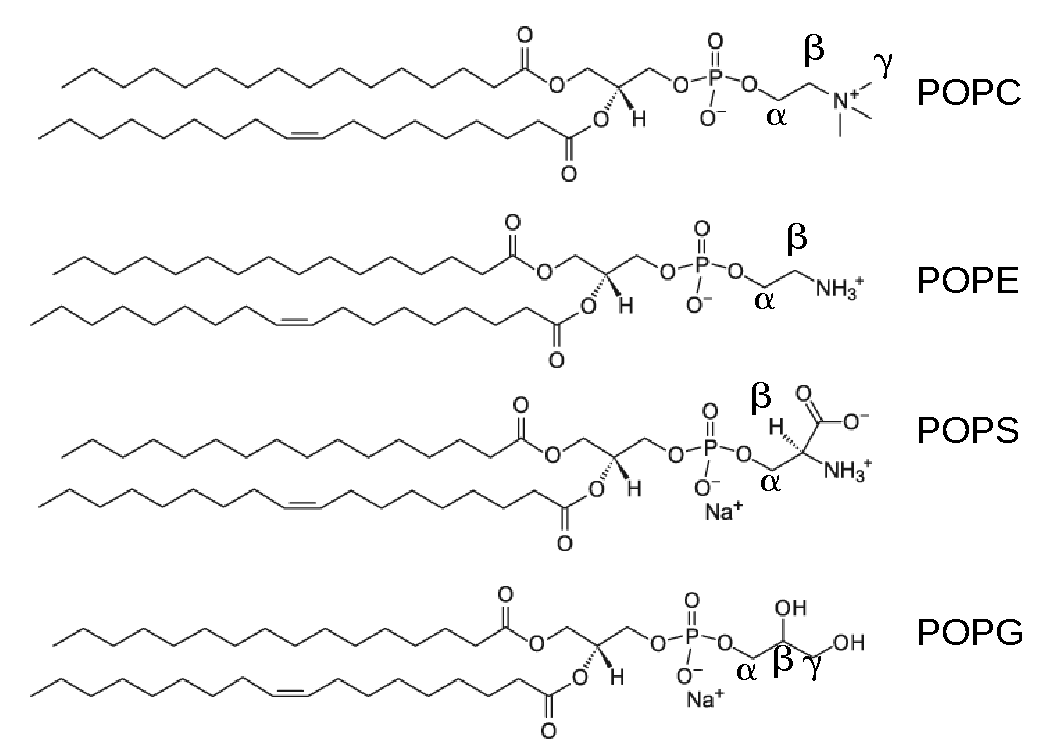
\includegraphics[width=9.0cm]{../Figs/lipids.pdf}
  \includegraphics[width=9.0cm]{../Figs/HGorderparametersPCPSPEPG.eps}
  \caption{\label{HGorderParameters}
    (top) Chemical structure of different lipids
    (bottom) Headgroup and glycerol backbone order parameters measured from lipids
    with different headgroups in lamellar liquid disordered phase.
    The values and signs for POPE (310~K), POPG (298~K). POPS (298~K) \cite{antila19} and POPC (300~K) \cite{ferreira13,ferreira16}
    are measured using $^{13}$C NMR. The literature values for
    DOPS with 0.1M of NaCl (303~K) \cite{browning80},
    POPG with 10nM PIPES (298~K) \cite{borle85},
    DPPG with 10mM PIPES and 100mM NaCl (314~K) \cite{wohlgemuth80}, 
    DPPE (341~K) \cite{seelig76},
    E.coliPE and E.coliPG (310~K) \cite{gally81}
    are measured using $^2$H NMR. The signs from $^{13}$C NMR are used also for the literature values.
  }
\end{figure}

In conclusion, the results suggests that the glycerol backbone conformations in all lipids are
relatively similar. Also, the headgroup conformations are similar for PC and PE lipids, while
PS and PG are singnificantly different. For PS lipids, the differences are discussed previously \cite{??}.

\subsection{Headgroup and glycerol backbone of POPE and POPG in MD simulations}
As reported previously for PC \cite{botan15} and PS \cite{antila19} lipids,
the headgroup and glycerol backbone order parameters show wide variation between different force fields
for both PE and PG lipids (Figs. \ref{HGorderParametersPE} and \ref{HGorderParametersPOPG}),
and none of the force fields reproduce all values within experimental error bars.
%The Slipid simulations were able to capture the essential differences between PC and PS lipid
%headgroups \cite{antila19}, but this is not the case for PE and PG lipids.
%\todo{Berger results are not here yet, but we should mention the ring like structures
%  pointed out by T. Piggot in the blog:
The poor performance of headgroup order parameters in Berger model can be probably explained by ring like structures seen in Fig. 6 in Ref. \citenum{mukhopadhyay04},
which is a typical feature for Berger based lipid force fields containing explicit hydrogen atoms in the head group \cite{zhao08,henin09,dahlberg10}.
%}


\begin{figure}[]
  \centering
  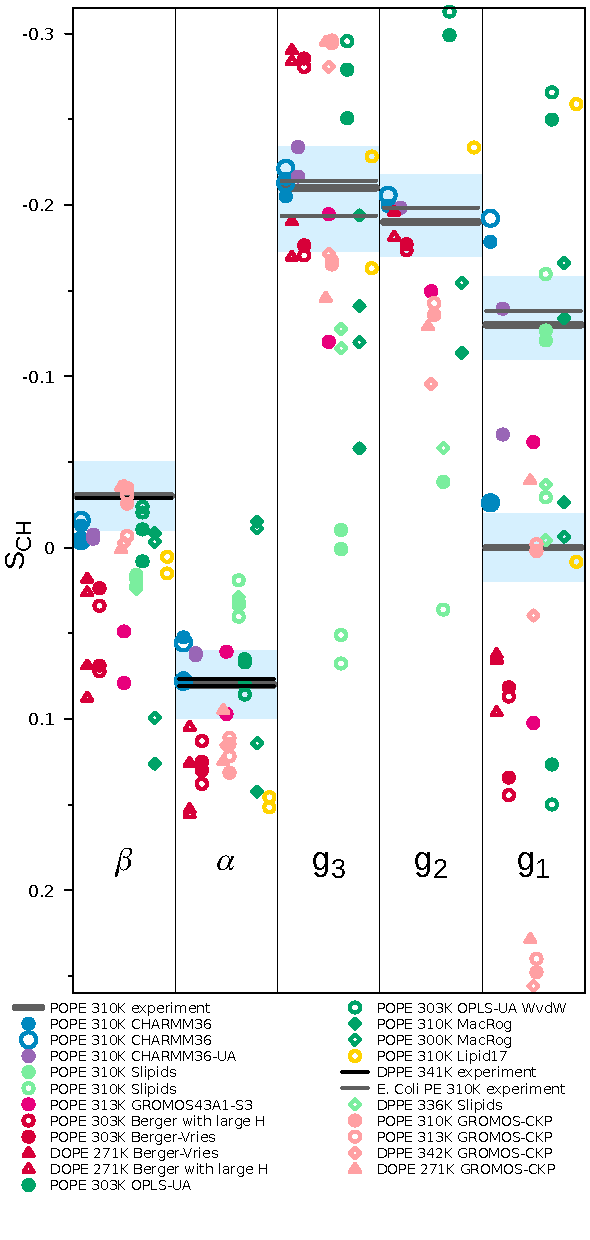
\includegraphics[width=9.0cm]{../Figs/HGorderparametersPE.pdf}
  \caption{\label{HGorderParametersPE}
    The headgroup and glycerol backbone order parameters of PE lipids
    from experiments (POPE and signs this work, DPPE from Ref.~\citenum{seelig76}
    and E.coliPE from Ref.~\citenum{gally81}) and simulations with different force fields.
  }
  \todo{This should be clarified as in NMRlipidsI and error bars should be added.
    Probably larger error bars for united atom models based on the report by Fuchs et al.
  }
\end{figure}

\begin{figure}[!h]
  \centering
  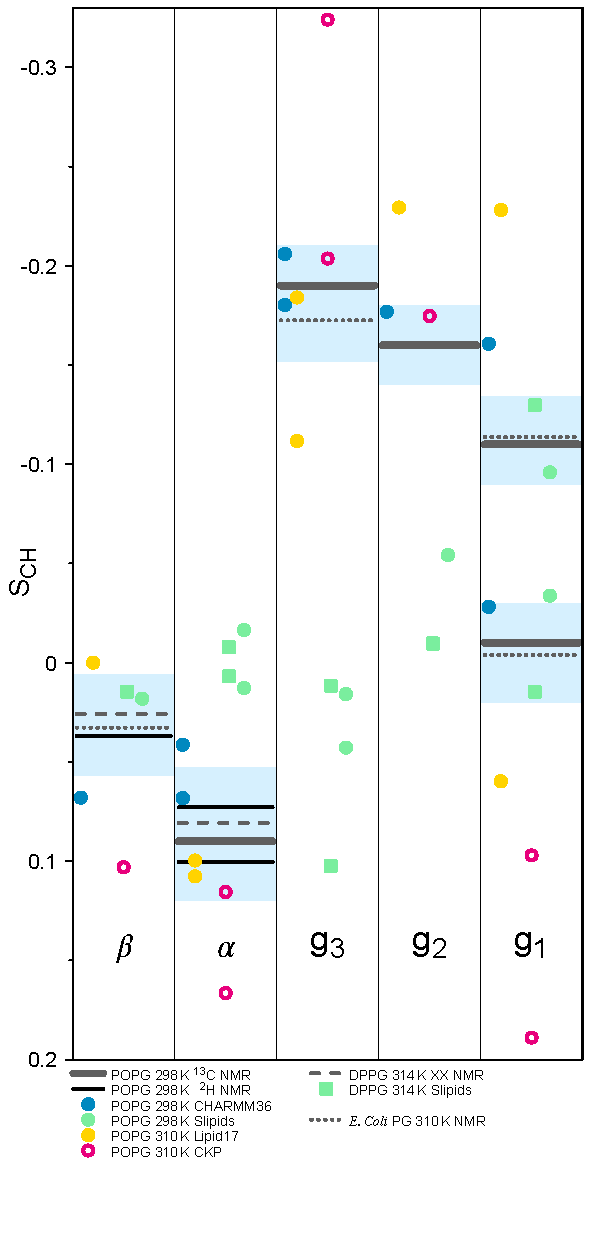
\includegraphics[width=9.0cm]{../Figs/HGorderparametersPG.pdf}
  \caption{\label{HGorderParametersPOPG}
    The headgroup and glycerol backbone order parameters of PG lipids
    from experiments (POPG and signs from this work and from Ref.~\citenum{borle85}, %contains 10mM of PIPES,
    DPPG with 100mM NaCl from Ref.~\citenum{wohlgemuth80},% contains 10mM PIPES and,
    and E.Coli PG results from Ref.~\citenum{gally81}).
    and simulations with different force fields.
  }
\end{figure}
\begin{figure*}[!h]
  \centering
  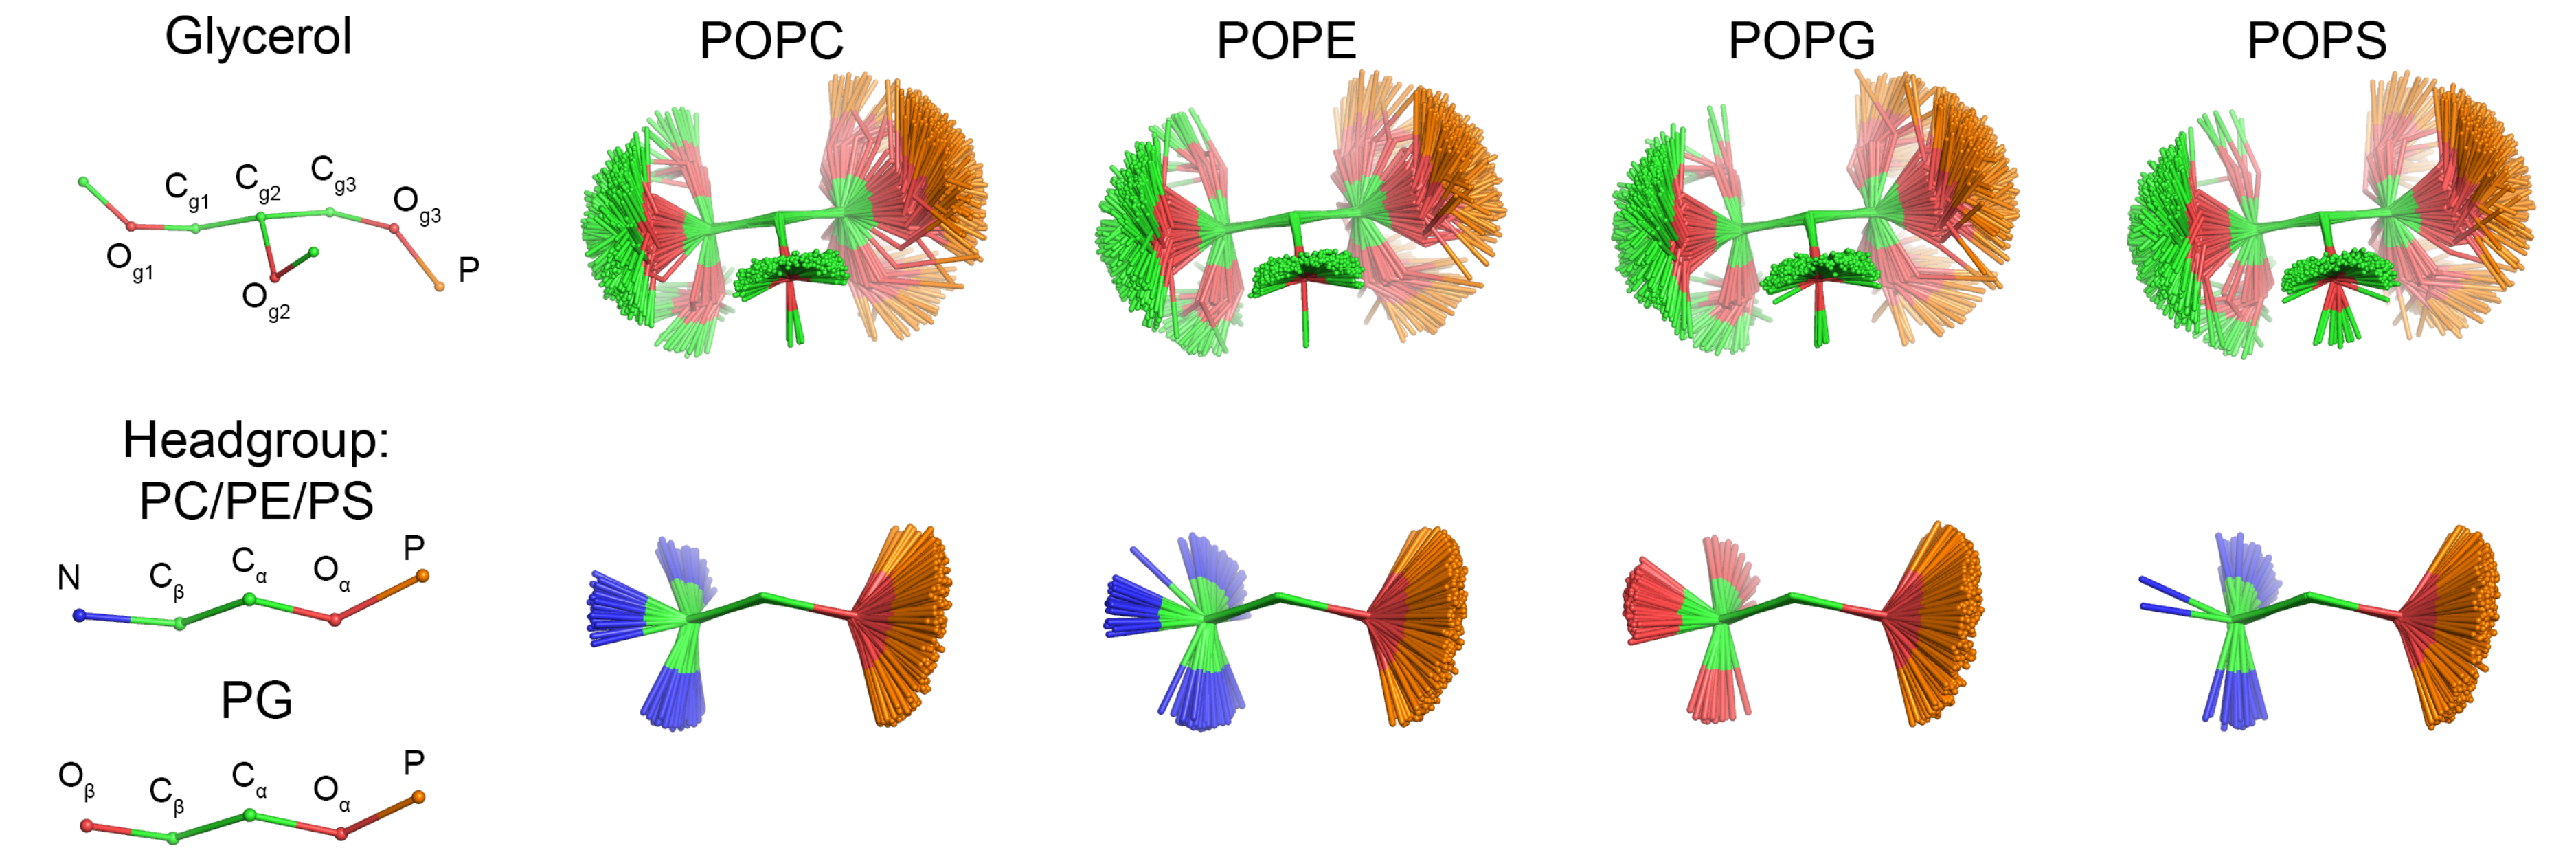
\includegraphics[width=18.0cm]{../Figs/struct.png}
  \caption{\label{structures}
    Overlayed snapshots from CHARMM36 simulations of different lipids which give the best agreement with experiments.
  }
\end{figure*}
Also in line with previous studies for PC \cite{botan15} and PS \cite{antila19} lipids,
CHARMM36 simulations are in best agreement with experiments for headgroup and glycerol backbone
order parameters, and seem to capture all the essential differences between different headroups
(Figs. \ref{HGorderParametersPE} and \ref{HGorderParametersPOPG}).
%headgroup order parameters of PC PE, PG (Figs. \ref{HGorderParametersPE} and \ref{HGorderParametersPOPG}),
%as previously observed also for PS lipids \cite{antila19}.
In previous study, CHARMM36 predicted the more negative $\beta$-carbon order parameter and larger forking of
the $\alpha$-carbon is PS headgroup than in PC \cite{antila19}.
In this work, the CHARMM36 simulations reproduce also the other essential differences in experimental
headgroup order parameters between different headgroups (Fig. \ref{HGorderParameters}) despite the inaccuracies
in individual segments:
The PE headgroup order parameters in CHARMM36 simulations are similar to the PC \cite{botan15}
and $\beta$-carbon order parameters is positive in PG headgroup, in contrast to the negative values observed in
other lipids. Therefore, we use CHARMM36 simulations to analyze the structural differences between
headgroups (Fig.~\ref{structures}). While rotation around N-C$_\alpha$-C$_\beta$-O$_\alpha$ dihedral was
significantly different in PS and PC headgroups in previous work \cite{antila19}, essential differences
between PC, PE and PG are not observed here (Fig.~\ref{structures}) \todo{We need also the dihedral distributions to finish this discussion.}. \\
\todo{Why is the $\beta$-carbon order parameter of PG different to PC and PE then?}

\subsection{PC headgroup interactions with PE and PG}
\begin{figure*}[]
  \centering
  \includegraphics[width=16.0cm]{../Figs/HGorderparametersPCvsPEPG.eps}
  \caption{\label{HGorderparametersPCvsPEPG}
    Modulation of POPC headgroup order parameters with increasing amount of POPE (left) and POPG (right) in bilayer
    from experiments \cite{scherer87,macdonald87} and simulations with different force fields.
    Signs are determined as discussed in \cite{botan15,ollila16}.
  }
  \todo{Data for CHARMM without ions to be added once this issue is solved: https://github.com/NMRLipids/MATCH/issues/83}
  %\todo{Simulation of CHARMM36 at 298K should be maybe rerun with Gromacs 5.}
\end{figure*}
According to the electrometer concept, the PC headgroup order parameters increase
with the addition of negatively charged PG or PS lipids, but
are not affected by the addition of zwitterionic PE and SM lipids
or cholesterol (Fig.~\ref{HGorderparametersPCvsPEPG}) \cite{seelig87, scherer87,antila18}. 
The different responses of PC headgroup order parameters to PE and PG are roughly
reproduced in CHARMM36 simulations, although the changes are slightly
overestimated upon addition of PE and underestimated upon addition of PG (Fig.~\ref{HGorderparametersPCvsPEPG}).
Interestingly, the response of POPC headgroup order parameters to POPE is
close to experiments also in Berger-OPLS simulations, even though the response
of Berger force field to cholesterol was significantly overestimated in our previous work \cite{botan15}.
In all force fields except Slipids, the $\alpha$-carbon order parameters of different
hydrogens are responsing differently when mixed with PE or PG lipids \todo{Maybe we should figure out what is the reason for this}.
\todo{Maybe we should analyze the P-N vector angle from different simulations}.

For $\beta$-carbon order parameter in PG headgroup, experiments report
mild increase \cite{macdonald87} or no change~\cite{borle85} upon addition 
of PC lipids (Fig. \ref{HGorderparametersPGvsPCchange}). 
Simulations with all the tested force fields give only very small changes also for
the $\alpha$-carbon order parameter (Figs. \ref{HGorderparametersPGvsPC} and \ref{HGorderparametersPGvsPCchange}). 
Therefore, the simulations are generally in line with experimetns, suggesting that the
interactions with PC do not essentially effect the PG headgroup structure.
This is in contrast with previous results for PS headgroup \cite{antila18}, where
all the force fieds significantly overestimated the structural response of PS headgroup
to the interactions with PC lipids.
\begin{figure}[]
  \centering
  \includegraphics[width=8.0cm]{../Figs/HGorderparametersPGvsPCchange.eps}
  \caption{\label{HGorderparametersPGvsPCchange}
    Modulation of PG lipid headgroup order parameters with the increasing amount of PC in lipid bilayer
    from experiments \cite{borle85,macdonald87} and simulations with different force fields.
  }
\end{figure}

\todo{This is text by P. Fuchs, copied from the blog. \\
Area results in nm$^2$, the error is $<=$ 0.003 nm$^2$ \\
- pure POPC \\
CHARMM36: 0.624 \\
Berger : 0.649 \\
- POPC/POPE 50:50 \\
CHARMM36 : POPC 0.609, POPE 0.557 \\
Berger-hacked: POPC 0.637, POPE 0.632 \\
----- \\
One can see that CHARMM 36 predicts a drop in the area on going from pure POPC to POPC/POPE 50:50. This means that POPC pack tightly to POPE. 
In contrast, the values for Berger are not that changed. 
The POPE value predicted by CHARMM 36 (in the mixture POPC/POPE 50:50) is much smaller than that predicted by Berger.\\
-------\\
The experimental acyl chain order parameters for POPE \cite{pare98} seem larger than reported for POPC \cite{ferreira13},
which supports the more condensed PE bilayer.
This is interesting, but to avoid the overexapansion of the manuscript, it is probably better to keep the focus in headgroups and ion binding also in this manuscript.}




\subsection{Sodium binding to PE and PG lipid bilayers}
In our previous study about PS lipids \cite{antila18}, the underestimated increase of PC
headgroup order parameters upon addition of negaticely charged lipids
was related
to the overestimated counterion binding affinity, which would overcompensates the effect of negative charge.
Similar correlation is observed here in %other than GROMOS-CKP simulation:
Lipid 17 simulations, which exhibits stronger counter-ion binding affinity to pure POPG bilayer (Fig. \ref{CIdensPG})
and larger decrease in POPC $\beta$ carbon order parameter upon addition of POPG than other simulations.
Together with the lower area per molecule (59.5 {\AA}$^2$) than in experiments (66.1 {\AA}$^2$),
the results suggest that the counterions bind too strongly and shield the electrostatic repulsion between PG headgroups
in bilayers simulated with Lipid17 parameters.
In GROMOS-CKP simulations, however, the $\beta$-carbon order parameter of POPC
increases upon addition of POPG more than in CHARMM36 and Slipids simulations even though the binding affinities in these
simulations are similar. On the other hand, the responses of different hydrogens attached in $\alpha$-carbons
are different in all simulations except in Slipids, most sever in Lipid17 and GROMOS-CKP where other in increases
and other decreases \todo{Can we figure out the reason for this?}.
In conclusion, the counter-ion binding seems to be overestimated in Lipid17 with the strongest affinity among the
tested models, while with this data we cannot fully evaluate binding affinity in the other models.
\begin{figure}[]
  \centering
  \includegraphics[width=9.0cm]{../Figs/CIdensPG.eps}
  \caption{\label{CIdensPG}
    Counterion densities and area per lipids from simulations with PG lipids.
    Experimental area for POPG at 303 K is 66.1 {\AA}$^2$ and 67 {\AA}$^2$ for DPPC at 323 K \cite{pan12b}.
  }
\end{figure}

%Sodium binding to PC lipid bilayers is significantly overestimated by most simulations models \cite{catte16}.
%Also, sodium binding to PS lipids seems to be overestimated, although the
%presence of counterions complicate the comparison for negatively charged lipids \cite{antila19}.
Similarly to POPG, the Lipid17 exhibits stronger sodium binding affinity
to POPE bilayers than Slipids, CHARMM36 and GROMOS-CKP (Fig. \ref{NAdensPE}).
In Lipid17 the sodium binding affinity to POPE is approximately similar as to POPC,
while in other models exhibit weaker binding to POPE (Fig. \ref{NAdensPC}).
The difference is small in Slipids and CHARMM36, while GROMOS-CKP predicts
subtantially stronger binding to POPC.
Experimental data for sodium binding to PE lipids is not available, while
simulations in agreement with electrometer data from NMR suggests that
sodium binding to POPC is weaker than in any of the simulations
here (Fig. \ref{NAdensPC})~\cite{catte16,melcr18}. Assuming that the binding
to POPE would be similar than to POPC, the sodium binding affinity to POPE
is potentially realistic in CHARMM36, Slipids, and GROMOS-CKP simulations here,
but substantially overestimated in Lipid17 simulation.
%On the other hand, the sodium binding affinity is stronger to POPE in Lipid17 simulations than to POPC in simulations with
%previous Amber lipid version, Lipid14.
\todo{The potential differences in the used ion models should be checked}.
\begin{figure}[]
  \centering
  \includegraphics[width=8.0cm]{../Figs/NAdensPE.eps}
  \caption{\label{NAdensPE}
    Sodium (solid line) and choride ion density profiles along membrane normal
    from different simulations with PE lipids.
  }
\end{figure}






\clearpage
\subsection{Cation binding to PE and PG lipid bilayers}
The headgroup order parameters of PC lipids can used to measure ion binding
affinity to lipid bilayers, because their magnitude is linearly proportional
to the amount of bound charge in bilayer according to the molecular
electrometer concept \cite{seelig87,catte16}. The molecular electrometer concept
can be used also for bilayers containing PC lipids mixed with charged
lipids \cite{borle85,macdonald87,roux90,antila19}.
%This is demonstrated in Figs \ref{OrderParametersWithCaCl},
%\ref{OrderParametersWithCaClBELOW1M} and \ref{OrderParameterCHANGESWithCaClBELOW1M},
%showing order parameters for PC headgroup $\alpha$ and $\beta$ carbons
%as a function of CaCl$_2$ concentration in the presence of different amounts of
%negatively charged PS or PG lipids.
%
%PC headgroup order parameters increase when negatively charged
%PS or PG are added to PC bilayer in the absense of added CaCl$_2$,
%as expected based on electrometer concept \cite{seelig87}
%(see Fig. \ref{OrderParametersWithCaClBELOW1M}).
%Further, the order parameters decrease with the addition
%of CaCl$_2$ and the decrease is more pronounced for systems with more
%negatively charged lipids (see Fig. \ref{OrderParameterCHANGESWithCaClBELOW1M}).
%At CaCl$_2$ concentrations ($\sim$ 50-300mM) where order parameters reach the values for pure PC,
%the Ca2+ binding presumably fully cancels the charge from negative lipids and
%overcharging occurs above these concenterations.
The electrometer concept has been very useful in evaluating ion binding affinity in simulations
against experiments, because the headgroup order parameter changes as a function of ion concentration
can be directly compared with experiments \cite{catte16,melcr18,antila19}.

Calcium binding affinity to PC and PS lipid bilayers was not correctly described by
any of the standard MD simulation forced fields \cite{catte16,antila19}, while
recently introduced force field with electronic continuum correction (ECC) performed better \cite{melcr18}.
The decrease of $\alpha$-carbon order parameter of PC lipids in PC:PG mixtures as a function
of calcium concentration is close to experiments CHARMM36 simulations (Fig. \ref{changesWITHCaClPG}),
but the decrease of $\beta$-carbon order parameter seems to be overestimated.
However, the $\beta$-carbon order parameter was not actually measured from these samples,
but they are calculated from empirical relation $\Delta S_{\beta}=0.43\Delta S_{\alpha}$ \cite{akutsu81}.
The result is similar to the $\sim$200~ns simulations with PC lipids in previous work \cite{catte16}.
However, when simulation was continued for $\mu$s, the binding affinity substantially increased
and interpretation was that calcium overbinds to PC lipid in CHARMM36. Therefore, the
conclusion seems to be similar here, although the new NBfix parameters may complicate
the situation \todo{The status of NBfix parameters in these simulations should be checked.}.
%Anyway, the data presented in NMRlipids II project and in Fig. \ref{changesWITHCaClPG} together
%suggest that Calcium binding is similarly overestimated by CHARMM36 model in pure POPC bilayers and mixtures with
%POPG. The good agreement of $\alpha$ carbon would be explained by too weak dependence of its order
%parameter of bound charge
%\todo{The response of CHARMM36 to cationic surfactant against experiments \cite{scherer89} to be checked.
%  I have already ran the simulations, analysis to be done.}.
\begin{figure*}[]
  \centering
  \includegraphics[width=18.0cm]{../Figs/CHANGESwithCaClPG.eps}
  \caption{\label{changesWITHCaClPG}
    (left) The headgroup order parameters of PC from PC:PG mixtures as a function CaCl$_2$
    concentration from experiments \cite{borle85,macdonald87} and CHARMM36 simulations.
    Note that beta order parameter is calculated from empirical relation $\Delta S_{\beta}=0.43\Delta S_{\alpha}$ \cite{akutsu81}, not actually measured.
    (right) The headgroup order parameters of PG from PC:PG mixtures as a function CaCl$_2$
    concentration from experiments \cite{borle85} and CHARMM36 simulations.
  }
\end{figure*}

The $\beta$-carbon order parameter of PG exhibits a rapid decrease with small CaCl$_2$ concentrations
and a more modest decrease with larger concentrations in experiments \cite{borle85} (Fig. \ref{PSPGchangesWITHCaCl}).
The rapid decrease with CaCl$_2$ is observed but overestimated in CHARMM36 simulation
with POPC:POPG 1:1 mixture, but not in 4:1 mixture \todo{This is little bit weird, should be checked.}.



\begin{figure}[]
  \centering
  \includegraphics[width=8.0cm]{../Figs/CAdensPG.eps}
  \caption{\label{CAdensPG}
    Calcium ion density profiles along membrane normal
    from different simulations with PG lipids.
  }
\end{figure}


\todo{We need PC:PG simulations with CaCl$_2$ from different force fields to finish the discussion.}



\section{Conclusions}


% Tables may be be put in the text as floats.
% Here is an example of the general form of a table:
% Fill in the caption in the braces of the \caption{} command. Put the label
% that you will use with \ref{} command in the braces of the \label{} command.
% Insert the column specifiers (l, r, c, d, etc.) in the empty braces of the
% \begin{tabular}{} command.
%
% \begin{table}
% \caption{\label{} }
% \begin{tabular}{}
% \end{tabular}
% \end{table}

% If you have acknowledgments, this puts in the proper section head.
\begin{acknowledgments}
% Put your acknowledgments here.
\end{acknowledgments}
\newpage
\appendix
\begin{center}
{\bf SUPPLEMENTARY INFORMATION}
\end{center}



%\section{Measurements of order parameter sign}

%Fig. \ref{PShgSIGNS} summarizes the experimental results on the order parameter sign
%measurement for POPS sample. The experimental protocol is the same used in Ref. \citenum{ferreira16}.
%In (a) you see the headgroup region of the INEPT spectrum where alpha and beta are
%identified. In (b) you have the R-PDLF slices for alpha and beta where you see one single
%splitting for beta (which gives an order parameter equal to 0.12), and for alpha a superposition
%of a large splitting (order parameter equal to 0.09) and a very small splitting which cannot be
%calculated. On the bottom you have the S-DROSS slices of these two carbons. The grey lines show a
%random collection of slices from noise such that it gets clear what is significant. The S-DROSS
%slice for beta clearly shows that the order parameter is negative. The slice for alpha shows that
%the higher order parameter is positive and suggests that the smaller order parameter is negative
%(from the deviation towards negative values in the longer t1 times).
%\begin{figure}[]
%  \centering
%  \includegraphics[width=9.0cm]{../Figs/PShgSIGNS.pdf}
%  \caption{\label{PShgSIGNS}
%    Experimental results for sign measurement for POPS sample
%  }
%\end{figure}

%The results updated with SIMPSON simulations for the SDROSS profiles
%are shown in Fig. \ref{PShgSIGNSsimpson}. The value for the smaller
%alpha order parameter is taken from Fig 3 in Ref. \citenum{roux91},
%because resolution in 13C NMR experiments was nor high enough to determine
%numerical value for this. The plots in Fig. \ref{PShgSIGNSsimpson} (c) show
%the following. The error bars and points are the experimental SDROSS data.
%The thick lines are SIMPSON simulations. The simulations were done by using
%the order parameter for beta equal to -0.12 and for alpha one order parameter
%equal to 0.09 and the other equal to -0.02 (black) or 0.02 (grey).
%Since the black lines agree with experimental data, we conlude that
%the order parameters for $\beta$ carbon are -0.12 and for $\alpha$
%order parameters are 0.09 and -0.02.
%\begin{figure}[]
%  \centering
%  \includegraphics[width=9.0cm]{../Figs/PShgSIGNSsimpson.pdf}
%  \caption{\label{PShgSIGNSsimpson}
%    Experimental results for sign measurement for POPS sample
%  }
%\end{figure}

%\section{Dihedrals}
%\begin{figure*}[]
%  \centering
%  \includegraphics[width=8.0cm]{../Figs/dihed1.png}
%  \includegraphics[width=8.0cm]{../Figs/dihed2.png}
%  \includegraphics[width=8.0cm]{../Figs/dihed3.png}
%  \includegraphics[width=8.0cm]{../Figs/dihed4.png}
%  \includegraphics[width=8.0cm]{../Figs/dihed5.png}
%  \includegraphics[width=8.0cm]{../Figs/dihed6.png}
%  \includegraphics[width=8.0cm]{../Figs/dihed7.png}
%  \includegraphics[width=8.0cm]{../Figs/dihed8.png}
%  \includegraphics[width=8.0cm]{../Figs/dihed9.png}
%  \includegraphics[width=8.0cm]{../Figs/dihed10.png}
%  \caption{\label{dihedrals}
%    Experimental results for sign measurement for POPS sample
%  }
%\end{figure*}

% Create the reference section using BibTe
\bibliography{refs.bib}

%\newpage
%\section{APPENDIX: The NMR results reported by Tiago Ferreira}

\listoftodos

\end{document}
%
% ****** End of file aiptemplate.tex ******
